% --- Template for thesis / report with tktltiki2 class ---
% 
% last updated 2013/02/15 for tkltiki2 v1.02

\documentclass[finnish]{tktltiki2}

% tktltiki2 automatically loads babel, so you can simply
% give the language parameter (e.g. finnish, swedish, english, british) as
% a parameter for the class: \documentclass[finnish]{tktltiki2}.
% The information on title and abstract is generated automatically depending on
% the language, see below if you need to change any of these manually.
% 
% Class options:
% - grading                 -- Print labels for grading information on the front page.
% - disablelastpagecounter  -- Disables the automatic generation of page number information
%                              in the abstract. See also \numberofpagesinformation{} command below.
%
% The class also respects the following options of article class:
%   10pt, 11pt, 12pt, final, draft, oneside, twoside,
%   openright, openany, onecolumn, twocolumn, leqno, fleqn
%
% The default font size is 11pt. The paper size used is A4, other sizes are not supported.
%
% rubber: module pdftex

% --- General packages ---

\usepackage[utf8]{inputenc}
\usepackage[T1]{fontenc}
\usepackage{lmodern}
\usepackage{microtype}
\usepackage{amsfonts,amsmath,amssymb,amsthm,booktabs,color,enumitem,graphicx}
\usepackage[pdftex,hidelinks]{hyperref}
\usepackage{graphicx}



% Automatically set the PDF metadata fields
\makeatletter
\AtBeginDocument{\hypersetup{pdftitle = {\@title}, pdfauthor = {\@author}}}
\makeatother

% --- Language-related settings ---
%
% these should be modified according to your language

% babelbib for non-english bibliography using bibtex
\usepackage[fixlanguage]{babelbib}
\selectbiblanguage{finnish}

% add bibliography to the table of contents
\usepackage[nottoc]{tocbibind}
% tocbibind renames the bibliography, use the following to change it back
\settocbibname{Lähteet}

% --- Theorem environment definitions ---

\newtheorem{lau}{Lause}
\newtheorem{lem}[lau]{Lemma}
\newtheorem{kor}[lau]{Korollaari}

\theoremstyle{definition}
\newtheorem{maar}[lau]{Määritelmä}
\newtheorem{ong}{Ongelma}
\newtheorem{alg}[lau]{Algoritmi}
\newtheorem{esim}[lau]{Esimerkki}

\theoremstyle{remark}
\newtheorem*{huom}{Huomautus}


% --- tktltiki2 options ---
%
% The following commands define the information used to generate title and
% abstract pages. The following entries should be always specified:

\title{Test Driven Developement-menetelmän tehokkuus ja laatu}
\author{Petri Pihlajaniemi}
\date{\today}
\level{Kandidaatintutkielma}
\abstract{Tiivistelmä.}

% The following can be used to specify keywords and classification of the paper:

%\keywords{avainsana 1, avainsana 2, avainsana 3}

% classification according to ACM Computing Classification System (http://www.acm.org/about/class/)
% This is probably mostly relevant for computer scientists
% uncomment the following; contents of \classification will be printed under the abstract with a title
% "ACM Computing Classification System (CCS):"
% \classification{}

% If the automatic page number counting is not working as desired in your case,
% uncomment the following to manually set the number of pages displayed in the abstract page:
%
% \numberofpagesinformation{16 sivua + 10 sivua liitteissä}
%
% If you are not a computer scientist, you will want to uncomment the following by hand and specify
% your department, faculty and subject by hand:
%
% \faculty{Matemaattis-luonnontieteellinen}
% \department{Tietojenkäsittelytieteen laitos}
% \subject{Tietojenkäsittelytiede}
%
% If you are not from the University of Helsinki, then you will most likely want to set these also:
%
% \university{Helsingin Yliopisto}
% \universitylong{HELSINGIN YLIOPISTO --- HELSINGFORS UNIVERSITET --- UNIVERSITY OF HELSINKI} % displayed on the top of the abstract page
% \city{Helsinki}
%


\begin{document}

% --- Front matter ---

%\frontmatter      % roman page numbering for front matter

\maketitle        % title page
\makeabstract     % abstract page

\tableofcontents  % table of contents

% --- Main matter ---

\mainmatter       % clear page, start arabic page numbering




\section{Johdanto}

%***Yleistä, miksi testataan***

Ohjelmistotestauksen tarkoituksena on parantaa ohjelman laatua havaitsemalla ja poistamalla virheitä ohjelmakoodissa. Edsger Dijkstran sanontaa mukaillen: testauksen avulla ei voida todistaa ohjelman olevan virheetön, mutta sillä voidaan todistaa virheiden olemassaolo \cite{Randell69}. Ohjelmaa testataan erilaisilla syötteillä, jonka jälkeen ohjelman toimintaa verrataan odotettuun oikeaan lopputulokseen. Jos lopputuloksissa on eroa, on testi löytänyt virheen \cite{Muccini08}.

%***Prosessista on paljon lisätietoa Whittakerin artikkelissa, ehkä sieltä lisää?***

Testien kirjoittajan on tunnettava ohjelman rakenne ja toiminta pystyäkseen suunnittelemaan ja kirjoittamaan testejä. Testin kirjoittamiseni on vaikea ja aikaa vievä prosessi, ja se vaatii kehittäjältä hyviä taitoja \cite{Whittaker00}.

Ohjelmiston testaus suoritetaan eri vaiheissa riippuen valitusta ohjelmistokehitysmenetelmästä. Vuonna 1970 Winston W. Roycen määrittelemä \emph{vesiputousmalli} (Waterfall Model) kuvaa ohjelmistokehityksen vaiheisiin eroteltuna prosessina: ensin analysoidaan vaatimukset ja suunnitellaan koko ohjelma tarkasti, sitten kirjoitetaan varsinainen ohjelmakoodi ja lopuksi tuotettu ohjelmakoodi testataan. Vaiheittaisissa menetelmissä (Incremental Model) edellinen vesiputousmalli on jaettu useisiin pienempiin palasiin; koko ohjelmaa ei siis tarvitse suunnitella ja toteuttaa kerralla noudattaen vesiputousmallin järjestystä, vaan ohjelman rakentuu pienemmistä osista jotka on suunniteltu ja toteutettu erikseen. Stoican ja kumppanien mukaan testaus on helppoa inkrementaalisissa menetelmissä, kun taas vesiputousmallissa testauksessa havaittujen virheiden korjaaminen voi olla hankaa. Ketterät (Agile Model) ohjelmistokehityksen menetelmät perustuvat inkrementaaliseen malliin. \cite{Stoica13}. Yksi erityisesti testaamiseen keskittyvät toimintapa on ketteriin malleihin perustuva \emph{Test Driven Development}. \cite{Crispin06}

Aion tutkielmassani tarkastella TDD:n toimivuutta kahdella mittarilla: laadulla ja tehokkuudella. Nämä mittari ovat erittäin epämääräisiä, joten ensin on tutkittava mitä ne oikeastaan tarkoittavat.


\section{Laadun käsitteestä}

Näkemys ohjelmiston laadusta riippuu siitä, keneltä sitä kysytään. Ohjelman loppukäyttäjä saattaa olla aivan eri mieltä tietyn ohjelman laadusta verrattuna ohjelmojaan. Tavallista kuluttajaa tuskin kiinnostaa esimerkiksi ohjelmakoodin luettavuus, mutta toisaalta se on muille ohjelmoijille tärkeä laatuominaisuus. Ohjelmistokehityksen laadun käsitettä määrittäessä tärkeää on myös tiedostaa erilaiset näkökulmat.

Barbara Kitchenham ja Shari Lawrence Pfleeger esittelivät vuonna 1996 viisi laatunäkökulmaa: transendentin, käyttäjän, teollisuuden, tuotteen ja arvon näkökulman \cite{Kitchenham96}. Näkökulmat perustuvat David Garvinin näkemyksiin laadun käsitteestä muilla aloilla, esimerkiksi filosofiassa.

Transendentti näkökulma (Transcendental View) pitää laatua mahdottomana määrittää tarkasti, mutta kuitenkin havaittavana ominasuutena \cite{Kitchenham96}. Tämän näkökulman perusteella laatua on vaikea mitata, vaan se on lähinnä filosofinen käsite jota voidaan arvioida vain subjektiivisten kokemusten perusteella

Käyttäjän näkökulma (User View) näkee tuotteen sen käyttäjän perspektiivistä. Laadukas tuote toteuttaa käyttäjän sille asettamat vaatimukset ja on vaivattomasti käytettävä \cite{Kitchenham96}. Näkökulma vastaa parhaiten tavallista loppukäyttäjää, ohjelman toimivuus ja soveltuvuus tilanteeseen on tärkeintä. TDD:n käsittely tästä näkökulmasta on hankalaa: jos ohjelma on toimiva ei loppukäyttäjälle ole merkitystä millaista toimintatapaa ohjelmoija on käyttänyt.

Teollinen näkökulma (Manufacturing View) käsittelee tuotteen kehitysprosessia. Standardeja käyttävä ja vaatimukset huomioiva ohjelmistotuotantoprosessi johtaa laadukkaaseen tuotteeseen \cite{Kitchenham96}. Perspektiivi nostaa ohjelman kehittäjien noudattamat työtavat tärkeään asemaan, mutta Kitchenhamin ja Pfleegerin mukaan näkökulma on ongelmallinen: liiallinen standardien noudattaminen voi johtaa huonoihin tuloksiin. Standardien noudattamista käytetään usein myyntivalttina, joten teollisesta näkökulmasta on tullut merkittävin perspektiivi ohjelmistokehityksessä \cite{Cote07}. TDD:n käyttö edellyttää menetelmän määrittämiä toimintatapoja, joten tämän näkökulman huomiointi on perusteltua. 

Tuotteen näkökulma (Product View) tutkii ohjelmaa itseään. Näkökulman mukaan ohjelmakoodin sisäiset laatuominaisuudet vaikuttavat suoraan ohjelman ulkoiseen laatuun. Näkökulman puolestapuhujien mukaan näkökulmaa on helpoin mitata, koska koodin ominaisuuksia voidaan mitata objektiivisesti \cite{Kitchenham96}. Näkökulma on mielestäni järkevin valinta TDD:n tutkimiseen.

Arvon näkökulma (Value-based View) huomio tuotteen arvon olevan riippuvainen sitä käyttävän ryhmään näkökulmasta. Ryhmillä on erilaiset käsitykset laadusta, joten voi olla vaikeaa tasapainottaa esimerkiksi käyttäjän ja teollisuuden näkökulmaa. Eri näkökulmia tasapainottamalla pyritään tuotteeseen, josta asiakas suostuu maksamaan mahdollisimman paljon valmiista ohjelmasta \cite{Kitchenham96}.  

\subsection{ISO 9126}

International Organization for Standardization eli ISO julkaisi vuonna 1991 ISO/IEC9126 ohjelmistokehitystä käsittelevän laatumallin (quality model). \cite{ISO9126}  ISO/IEC9126 malli toteuttaa Kitchenhamin ja Pfleegerin perspektiivit \cite{Cote07}  ja se on yksi suosituimmista laatustandardeista \cite{Botella04}. ISO9126:n perustuu myös uudempi ISO25010-standardi joka tunnetaan myös nimellä SQuaRE. \cite{ISO2011}

 ISO9216 jakaa ohjelman laatuominaisuudet luokkiin joilla on alaluokkia. Alaluokkiin sisältyy erilaisia ominaisuuksia, joita voidaan mitata metriikoilla. Luokkien, alaluokkien ja ominaisuuksien kokonaisuus muodostaa monikerroksisen hierarkian.\cite{Miguel14} Nämä ominaisuudet on jaettu kolmeen osaan, sisäiseen laatuun, ulkoiseen laatuun ja käyttölaatuun. Standardin mukaan osat muodostavat kokonaisuuden, jossa eri osissa tehdyt ratkaisut vaikuttavat ja riippuvat muiden osien laatuun, esimerkiksi ulkoinen laatu on riippuvainen sisäisestä laadusta.


%Tästä saa paljon täytettä kun selittää alaluokkia paremmin... nyt ihan hirveän kankeaa.

Sisäisellä laadulla tarkoitetaan koodin laatuominaisuuksia, esimerkiksi rakennetta ja luettavuutta. Ulkoinen koodi viittaa ohjelman toimintaan sitä ajettaessa, esimerkiksi virheiden määrään. ISO9216 jakaa sisäisen ja ulkoisen laadun osien luokiksi toimivuuden, luotettavuuden, käytettävyyden, tehokkuuden, ylläpidettävyyden ja siirrettävyyden. Kaikkiin luokkiin sisältyy useita alaluokkia.

Toimivuus (Functionality): ohjelman kyky vastata sille asetettuihin vaatimuksiin.  Luokan alaluokkia ovat soveltuvuus tehtävään, ohjelman antamien tuloksien oikeellisuus, toiminta muiden ohjelmien kanssa, turvallisuus sekä standardien, kuten lakien, noudattaminen. Testivetoinen kehitys vaikuttaa myös ohjelman rakenteeseen, joten uskoisin menetelmän vaikuttavan positiivisesti tähän tekijään.

Luotettavuus (Reliability): kuinka ohjelmisto säilyttää suoritustason erilaisissa tilanteissa. Kypsyys, eli virheistä johtuvien häiriöiden välttäminen, virheiden sietäminen, virheistä palautuminen sekä luotettavuuteen liittyvien standardien noudattaminen. Yksi TDD:n tärkeimmistä esitetyistä ominaisuuksista on testien laajuus ja kattavuus, joten uskon tekniikan tuomien hyötyjen vaikuttavan erityisesti tähän kategoriaan.

 Käytettävyys (Usability): ohjelman helppokäyttöisyys ja miellyttävyys. Ymmärrettävyys, ohjelman opittavuus, käytettävyys, viehättävyys ja käytettävyysstandardien noudattaminen. Testivetoinen kehitys ei ota kantaa käyttöliittymän käytettävyyskysymyksiin, joten epäilen TDD:n vaikuttavan mitenkään käytettävyyteen.

Tehokkuus (Efficiency): kuinka hyvin ohjelma toimii erilaisilla resursseilla. Luokan alaluokkia ovat ajankäyttö, eli kuinka ohjelman vasteaika muuttuu erilaisissa ympäristöissä, resurssien hyödyntämisen tehokkuus sekä tehokkuusstandardien noudattaminen. TDD:n käyttö parantaa todennäköisesti ohjelman rakennetta, joka saattaa vaikuttaa hieman myös tehokkuuteen.

Ylläpidettävyys (Maintainability): mahdollisuudet muuttaa ohjelmaa. Alaluokkina analysoitavuus, muutettavuus, stabiilisuus, testattavuus ja ylläpidettävyysstandardien noudatus. Testivetoinen kehitys pakottaa kehittäjän suunnittelemaan metodeita pieninä osina välttäen liiallista toiminnallisuutta ja refaktoroimaan koodia, tämä luultavasti parantaa myös ylläpidettävyyttä.

Siirrettävyys (Portability): ohjelman siirrettävyys alustalta toiselle, esimerkiksi eri käyttöjärjestelmälle. Sopeutuvuus, eli kuinka helposti ohjelmaa voidaan muuttaa toiselle alustalle sopivaksi, asennettavuus, rinnakkaiselo muiden ohjelmien kanssa, korvattavuus, eli toiminta jonkun toisen ohjelman tilalla, sekä siirrettävyysstandardien noudatus. Mielestäni testivetoisen kehityksen menetelmä ei vaikuta tähän ominaisuuteen käytännössä mitenkään.


Käyttölaatu (Quality in use) viittaa ISO:n standardissa valmiin tuotteen käyttöön. Tuotteen loppukäyttäjän kokemusta mitataan tehokkuudella, tuottavuudella, turvallisuudella ja tyytyväisyydellä.

%Saa paljon paremmaksi kun käy läpi artikkelin viitteet ja ottaa niistä kuvaukset





\subsection{Laadun mittareita}

Erilaisia tapoja mitata laatua esiintyy kymmeniä erilaisia tieteellisissä julkaisuissa. Shyam R. Chidamber ja Chris F. Kemerer esittelivät vuonna 1994 olio-ohjelmoinnin arviointiin kehittelemänsä kuusi mittaria.\cite{Chidamber94}. Tibor Gyimóthy, Rudolf Ferenc, ja István Siket ovat puolestaan arvioineet näiden mittareiden toimivuutta avoimen lähdekoodin Mozilla-ohjelmistopaketin virheiden ennustamiseen \cite{Gyimothy05}. Michaelin ja kumppanien mukaan Chidamberin ja Kemenerin mittarit ovat yleisimmin viitatut olio-ohjelmoinnin mittarit \cite{Michael02}.

%kokeillaas tätä listaa
%Mittarin esittelyihin lisätään vielä Gyimothyn näkemys onko mittari toimiva

\begin{itemize}

  \item \textbf{Metodeita per luokka} (Weighted Methods Per Class). Mittaa metodien määrää luokassa. Metodien määrä ja monimutkaisuus vaikuttaa luokan ylläpidon hankaluuteen ja suuren määrän metodeita sisältävä luokka on hankalampi käyttää uudelleen \cite{Chidamber94}. Gyimóthy ja kumppanig havaitsivat luokan jolla määrä on korkea olevan virhealttiimpi kuin luokan jolla määrä on matala. \cite{Gyimothy05}

  \item \textbf{Perintäpuun syvyys} (Depth of Inheritance Tree). Kuinka monta ylempää luokkaa luokalla on. Mitä syvemmällä perintäpuussa luokka on, sen enemmän se perii metodeita. Syvät puut ovat monimutkaisempia ja alttiimpia virheille \cite{Chidamber94}. Perintäpuussa syvällä oleva luokka on virhealttiimpi, mutta se ei ole yhtä hyvä mittari kuin jotkut muista tutkituista. \cite{Gyimothy05}

  \item \textbf{Lasten määrä} (Number of Children). Kuinka monta alaluokkaa luokalla on. Luokka jolla on paljon lapsia, vaatii paljon testausta. Luokka jolla on paljon aliluokkia on koodin uudelleenkäyttöä, toisaalta jos aliluokkia on paljon voi kyseessä olla aliluokkien väärinkäyttö \cite{Chidamber94}. Lasten suuren määrän ei havaittu olevan merkittävä mittari virheiden ennustamiseen. \cite{Gyimothy05}

  \item \textbf{Luokkien väliset kytkennät} (Coupling Between Object Classes). Luokat ovat kytketty, jos ne käyttävät toistensa metodeja tai muuttujia. Liiallinen kytkentä heikentää modulaarista suunnittelua ja vaikeuttaa uudelleenkäyttöä. Moneen luokkaan kytkettyä luokkaa pitää testata enemmän \cite{Chidamber94}. Kytkentöjen vähäinen määrä oli merkittävä, Gyimothyn ja kumppanien tutkimuksessa merkittävin ja paras, mittari \cite{Gyimothy05}.

  \item \textbf{Vastausten määrä} (Response For a Class). Kuinka monta metodia ajetaan vastauksena luokalle tulleeseen viestiin. Virheiden korjaus on hankalaa, jos ajettavia metodeita on paljon ja luokka on monimutkainen \cite{Chidamber94}. Suuren määrän vastauksia sisältävä luokka oli merkittävästi virhealttiimpi. \cite{Gyimothy05}

  \item \textbf{Metodien välisen koheesion puute} (Lack of Cohesion on Method). Mittaa luokasta löytyviä metodeita joilla ei ole yhteisiä muuttujia. Tavoite on siis se, että saman luokan metodit käsittelevät samoja muuttujia. Jos mittari havaitsee heikon koheesion, olisi kannattavaa pilkkoa luokka pienemmiksi osiksi \cite{Chidamber94}. Matalan koheesion luokat havaittiin virhealttiimmiksi. \cite{Gyimothy05}

  \item \textbf{Rivien määrä} (Lines of Code). Luokan koodirivien määrä.  Luokka jossa on suuri määrä koodirivejä on virhealttiimpi. Mittari oli toisiksi paras Gyimothyn ja kumppanien tutkimista mittareista, paljon koodirivejä sisältävissä luokissa oli enemmän virheitä. \cite{Gyimothy05}


\end{itemize}





\subsection{Tehokkuuden arviointi}

Aion tarkastella tehokkuutta testien perusteella, tehokas testimenetelmä löytää mahdollisimman suuren osan ohjelman virheistä pienimmällä mahdollisella vaivalla. Useissa ohjelmistokehitystä ja testausta käsittelevissä artikkeleissa on kuitenkin käytetty kahta eri termiä, effectiveness ja efficiency.  Effectiveness viittaa kykyyn saavuttaa lopputulos, efficiency taasen lopputuloksen saavuttamiseen vaadittuun aikaan ja vaivaan. Aionkin erotella nämä kaksi merkitystä tehokkuudeksi ja taloudellisuudeksi. Tehokkuudella tarkoitan esimerkiksi testien kattavuutta ja taloudellisuudella testien kattavuutta verrattuna aikaan ja vaivaan. Suurin osa testauksesta tehdyistä tutkimuksista määrittelee termit samalla tavalla kuin edellä. \cite{Juristo06}

Rothermel ja Harrold määrittelevät taloudellisuuden regressiotestaustatekniikoita käsittelevässä artikkelissaan \cite{Rothermel96} laskentatehon kulutukseksi. Tällainen määritelmä on testivetoista kehitystä käsittelevässä tutkielmassa mielestäni melko merkityksetön: jos testien ajaminen ylipäätään onnistuu on sen nopeudella vähäinen merkitys. Eldh ja kumppanit laajentavat Rothermelin ja Harroldin termin käsittämään myös testitapauksen ymmärtämisen ja luomiseen kuluvan ajan \cite{Eldh06}.

Rothermel ja Harrold käyttävät myös termejä sisältyvyys (inclusiveness), tarkkuus ja yleisyys. Sisältyvyydellä  tarkoitetaan kuinka hyvin käytetty ohjelmistotestaustekniikka valitsee virheiden löytämiseen sopivat testi. Tarkkuus mittaa kuinka paljon tekniikka pystyy välttämään turhien, virheitä löytämättömien, testien kirjoittamista. Yleisyys viittaa tekniikan kykyyn toimia erilaisissa tilanteissa, esimerkiksi käyttäessä monimutkaisia rakenteita.\cite{Rothermel96}

Frøkjær ja kumppanit määrittelevät tehokkuuden käyttäjän ohjelmalla saavuttamien tavoitteiden tarkkuudeksi ja täydellisyydeksi \cite{Frokjaer00}, heidän artikkelinsa tosin käsittelee termejä käytettävyyden perspektiivistä. Eldhin ja kumppanien näkemys tehokkuudesta testauksen näkökulmasta on yksinkertaisesti tekniikan löytämien virheiden määrä \cite{Eldh06}.



Yleisesti ottaen termit tehokkuus ja taloudellisuus tuntuvat tarkoittavan eri asioita eri artikkeleissa. Lukemissani TDD:tä käsittelevissä tutkimuksissa kuitenkin tehokkuudella on useimmiten tarkoitettu vertailua kulutetun ajan ja testien kattavuuden suhteesta. 





\section{Test Driven Development}

%Mikä se on, kuka keksi, miksi keksi? Paljonko käytetään?

Test Driven Development on Kent Beckin "löytämä" ohjelmistokehitystekniikka \cite{Beck03}. Menetelmästä käytetään myös termiä Test First Development \cite{Crispin06}. Suomenkieliseksi vastineeksi TDD:lle on muodostunut testivetoinen kehitys, mutta myös termiä testilähtöinen kehitys käytetään. Menetelmän perusideana on luoda ensin ohjelmalle testitapaus, ja sen jälkeen luoda testitapauksen läpäisevä osa ohjelmaa. Menetelmä on osa ketteriä menetelmiä, ryhmää ohjelmointitekniikoita joissa kehitys tehdään lyhyissä osissa. Tekniikan kulku Beckin menetelmässä on seuraava:

\begin{figure}[ht]
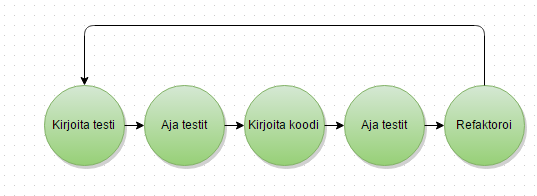
\includegraphics{tdd}
\end{figure}

\begin{enumerate}

  \item Kehittäjä tutkii esimerkiksi vaatimusmäärittelyn käyttötapauksia, ja kirjoittaa niiden perusteella testin.

  \item Kehittäjä ajaa testit ja varmistaakseen antaako ohjelma testin vaatiman lopputulokset ilman muutoksia. Testi saattaa myös mennä läpi vaikkei kehittäjä ole mielestään kirjoittanut koodia kyseiselle tapaukselle, tällöin laadittu testi saattaa olla virheellinen antaen aina hyväksytyn tuloksen.

  \item Jos testejä ei läpäisty, siirrytään kirjoittamaan koodia. Kehittäjä täydentää ohjelmaa antamaan hyväksyttävän tuloksen hylättyyn testiin. Lisätyn koodin pitäisi keskittyä ainoastaan testin määrittelemiin toimintoihin, tarkoitus ei ole kirjoittaa muuta toiminnallisuutta.

 \item Testit ajetaan uudestaan. Jos testi yhä epäonnistuu, palataan kohtaan kolme ja koodi parannellaan. Jos testi läpäistään, siirrytään seuraavaan kohtaan.

 \item Kirjoitettu koodi refaktoroidaan. Koodista esimerkiksi poistetaan turha toisto ja mahdollisesti ylipitkiksi kasvaneet metodit pilkotaan. Tämän jälkeen palataan ensimmäiseen kohtaan ja prosessi aloitetaan alusta uudella testillä.

\end{enumerate}

Testivetoisen kehityksen testit kirjoitetaan tutkimaan ohjelman pienimpiä mahdollisia yksikköjä, eli ohjelman osia joita voidaan testata \cite{Crispin06}. Crispinin mukaan pienimmän mahdollisen yksikön määritelmä on kiistanalainen, mutta olio-ohjelmoinnissa sitä on yleisesti pidetty metodina. Testien kirjoittaminen vasta varsinaisen koodin jälkeen voi kestää minuuteista kuukausiin, kun taas test driven developmentia käyttäessä testit ovat käytettävissä välittömästi. \cite{Janzen05}. 

Testivetoisen kehitys siis perustuu testaukseen, mutta se viekkaasti myös vaikuttaa suunnitteluun. Koska testit kirjoitetaan ensin, ohjelmoija joutuu miettimään miten toteuttaa koodi siten, että se on myös testattava. Menetelmä myös  kehottaa refaktoroimaan koodia säännöllisesti jokaisen kierroksen lopussa.

TDD:llä on myös muutamia samankaltaisia sukulaisia, esimerkiksi 
Acceptance Test Driven Development, Behavior-Driven Development ja Story-Test-Driven Development \cite{Turhan10}.


\section{Tutkimuksia}

Test Driven Development-menetelmästä on tehty useita tutkimuksia. Esimerkiksi Rafique ja kumppanit ovat tutkineet 27 empiiristä ennen helmikuuta 2011 julkaistua tutkimusta aiheesta \cite{Rafique13}. Turhan ja kumppanit löysivät peräti 325 artikkelia, joista he siivilöivät 22 tarkoituksenmukaista tutkimusta \cite{Turhan10}. 

Testivetoinen kehitys on siis tutkimusten määrästä päätellen kiinnostanut myös akateemisia tahoja.

%Tähän erilaisia tutkimuksia, mitä mittareita niissä on käytetty, millaiset tutkimusryhmät, mitä tuloksia


%Toimiiko vai ei?

\subsection{Laatu}

Päättelyni mukaan testivetoinen kehitys vaikuttaa positiivisesti ohjelmiston laatuun. Testien kirjoittaminen ennen ohjelmakoodia vaikuttaa varmistavan testikattavuuden lisäksi myös tarkemman rakenteen suunnittelun. Aiemmin artikkelissa esitellyistä laatutekijöistä testikattavuus ja parempi rakenne vaikuttavat mielestäni erityisesti ylläpidettävyyteen ja luotettavuuteen. Aion tarkastella TDD:stä kirjoitettujen artikkelien tuloksia ISO 9126:n määrittelemien sisäisen ja ulkoisen laadun kategorioiden perusteella, vaikka erilaisia tuloksia onkin vaikea lokeroida luokkien sisälle: onko esimerkiksi virheiden määrä ohjelmassa luotettavuuteen vai toimivuuteen littyvä termi? 

\subsubsection{Toimivuus}

En ole vielä löytänyt TDD:llä tuotettujen ohjelmistojen toimivuuteen liittyviä tutkimuksia. Yksi ongelma on englanninkielinen termi functionality, jolla usein TDD:tä käsittelevissä artikkeleissa viitataan ohjelman osien, kuten metodien, toimintaan. ISO:n laatustandardi kuitenkin määrittelee toimivuuden ohjelman toimivuudeksi, joten tutkimusten tapa käyttää termiä ei sovellu selkeästi tähän luokkaan. TDD:n väitetyt parannukset ohjelman rakenteen laatuun saattavat vaikuttaa toimivuuteen, mutta mielestäni tutkimukset aiheesta asettuvat loogisemmin muihin laatukategorioihin.

\subsubsection{Luotettavuus}

Luotettavuus vaikuttaa olevan suosituin laadun osa testivetoista kehitystä käsittelevissä artikkeleissa. Useat testit ovat mitanneet TDD:llä tuotetun ohjelmiston laatua testien läpäisyn perusteella, jota pidän lähinnä luotettavuuteen liittyvänä tekijänä. Toisaalta ISO:n laatuluokitusten mukaan luotettavuus voidaan ymmärtää myös tarkoittavan virheistä palautumista, eikä niinkään virheiden vähyyttä. ISO 9126-3 kuitenkin esittää koodikattavuuden ja katselmoidusta koodista havaittujen virheiden määrän luotettavuuden mittareina, joten mielestäni virheiden havaitsemiseen perustuvat tutkimukset ovat tässä osiossa perusteltuja.

Georgen ja Williamsin \cite{George04} tutkimuksessa havaittiin TDD:tä käyttäneiden parien tuottamien ohjelmien läpäisevän 18\% enemmän tutkijoiden rakentamia testitapauksia kuin kontrolliryhmien. Tutkimuksessa oli kuitenkin ongelmia joiden takia pidän tulosta kyseenalaisena: Georgen ja Williamsin tutkimuksessa ohjelmat olivat erittäin lyhyitä, pituudeltaan n. 200 riviä, ja suurin osa kontrolliryhmistä ei ollut tehnyt minkäänlaisia testejä ennen ohjelman palautusta tutkijoille.

Wilkersonin ja kumppanit \cite{Wilkerson12} vertailevat TDD:tä Code Inspection-menetelmään, jossa erillinen ryhmä katselmoi koodia. Tutkijoiden mukaan menetelmillä on selvä ero, katselmointi poistaa ohjelmasta löytyviä virheitä, mutta TDD käsittelee ne joi kehitysvaiheessa. Tutkimuksen tulosten mukaan katselmointia ja TDD:tä yhdistävän ryhmän ohjelmassa oli vähiten virheitä kun taas pelkkää TDD:tä käyttäneellä ryhmällä tulos ei ollut perinteisiä menetelmiä parempi. Tulos on mielestäni yllättävä, Wilkersonin ja kumppanien mukaan se saattaa selittyä TDD-menetelmän liian epämääräisellä määrittelyllä.

Erdogmus, Morisio ja Torchiano \cite{Erdogmus05} tutkivat testivetoista kehitystä verrattuna testien kirjoittamiseen jälkeenpäin (Test-Last). Tutkimuksen osaanottajista TDD:tä käyttäneet olivat kirjoittaneet keskimäärin 28 prosenttia enemmän testejä. Ohjelman laadussa testivetoinen kehitys olikin yllättäen jälkeenpäin testausta huonompi: Test-Last ryhmän mediaani virheiden määrässä käytettäessä tutkijoiden laatimaa testipakettia oli kymmenen prosenttia pienempi. Pidän tutkijoiden ehdottamaa selitystä TDD:n hieman heikomman laadun johtumisesta ohjelman pienuudesta ja koehenkilöiden erilaisista taitotasoista hyvänä. Testihenkilöiden tuottama ohjelma oli keilauksen pistelaskujärjestelmä, joka on mielestäni sen verran yksinkertainen tehtävä, että virheet pystyy helposti löytämään myös ilman yhtäkään automaattista testiä. Causevicin ja kumppanien \cite{Causevic12} tutkimus oli menetelmiltään hyvin samankaltainen kuin Erdogmusin ja kumppanien. Tässäkin tutkimuksessa vertailtiin keilailun pistelaskua suorittavan ohjelman testauksen laatua Test-First ja Test-Last menetelmillä käyttäen testiryhmänä yliopisto-opiskelijoita. Causevicin ja kumppanien tutkimuksessa molempien ryhmien testien laatu oli hyvin samankaltainen, eikä merkittäviä eroja havaittu. Itse ohjelman koodin laadussa oli kuitenkin ero TDD:n hyväksi. Vaikka tutkimukset olivat lähes identtiset,  oli tuloksissa pieni ero. Epäilen ohjelman ja koeryhmien pienuuden vaikuttavan näissä tutkimuksissa tulokseen enemmän kuin ohjelmointimenetelmän.

 Canfora ja kumppanit \cite{Canfora06} ovat testanneet menetelmää Espanjalaisen IT-yrityksen ammattilaisilla. Tutkijoiden mukaan TDD:n testit eivät ole tilastollisesti merkittävästi tarkempia vesiputousmallilla tuotettuihin verrattuna. Canfora ja kumppanit kuitenkin toteavat olevansa "vakuuttuneita" TDD:n positiivisesta vaikutuksesta laatuun, mutta heidän tutkimuksensa oli kenties liian lyhyt.

Pancur ja Ciglaric \cite{Pancur11} havaitsivat TDD:n tuottavan paremman päätöskattavuuden kuin iteratiivinen Test-Last menetelmä. Mutaatiotestauksessa ja hyväksyttyjen testien määrässä ei havaittu eroa. Myös Munirin ja kumppanien \cite{Munir14} tutkimuksessa päätöskattavuus oli parantanut, mutta tulos ei ollut tilastollisesti merkittävä johtuen liian pienestä koeryhmästä.

Nagappan ja kumppanit \cite{Nagappan08} tutkivat TDD:n vaikutusta laatuun ja tehokkuuteen IBM:n ja Microsoftin ohjelmistotuotannossa. Tutkijat määrittelivät laadun koodin virhetiheydeksi, ja virheiden määrä verrattuna samankaltaisiin projekteihin joissa TDD:tä ei oltu käytetty oli selvästi matalampi. IBM:n projekteissa vähennys oli 40\% ja Microsoftin projekteissa 60-90\%. Mielestäni tulokset ovat epäilyttävän hyviä, muissa tutkimuksissa en ole nähnyt näin radikaaleja muutoksia virhetiheydessä. Tutkijoiden mukaan tulos saattaa selittyä esimerkiksi projektien vaikeustasossa: TDD ryhmille on saattanut osua helpompia tutkimuksia.

\subsubsection{Käytettävyys}

Testivetoinen kehitys tuskin vaikuttaa loppukäyttäjän kokemukseen ohjelman laadusta. TDD ei varsinaisesti ota kantaa käytettävyyteen, eikä menetelmä sovellu graafisten käyttöliittymien suunnitteluun. Hellman ja kumppanit \cite{Hellman10} pitävät GUI:n kehitystä TDD:llä niin vaikeana, että ovat artikkelissaan pyrkineet kehittämään TDD:stä paremmin tehtävään sopivaa muunnosta.

En ole löytänyt tutkimuksia testivetoisen kehityksen vaikutuksesta käytettävyyteen, joten vertailenkin tässä osiossa itse menetelmän käytettävyyttä. TDD:n prosessi on yksinkertainen, joten uskon aloittelevankin ohjelmoijan ymmärtävän sen toimintatavat nopeasti. Olen hyväksynyt tähän osioon ainoastaan sellaisia tutkimuksia. Useissa tutkimuksissa käyttäjien omia näkemyksiä menetelmästä on selvitetty, mutta tähän osioon olen hyväksynyt vain tutkimuksen jossa TDD:n käytön oikeellisuutta on mitattu muutenkin kuin käyttäjien mielipiteiden perusteella.

Latorren \cite{Latorre14} tutkimuksessa mittauksien mukaan menetelmä oli helppo oppia, varsinkin kehittyneet ja keskitason ohjelmoijat oppivat sen nopeasti.

Oulun yliopiston Fucci, Turhan ja Oivo \cite{Fucci14} tutkivat TDD:n prosessin noudattamisen tarkkuuden vaikutusta laatuun. Fuccin ja kumppaneiden mukaan TDD:tä koskevissa tutkimuksissa menetelmän seuraamisen arviointi ei ole tehty tarpeeksi, vaikka se saattaa oleellisesti vaikuttaa tuloksiin. Tutkimuksen TDD:tä käyttäneiden opiskelijoiden tuottama laatu ei ollut ollut sidoksissa siihen, kuinka hyvin he noudattivat menetelmää. Tutkijat havaitsivat opiskelijoiden usein keskittyvän vain testien kirjoittamiseen ja jättävän refaktorointivaiheen kokonaan pois. Fucci ja kumppanit kyseenalaistavat TDD:n opettelun ja noudattamisen hyödyn, mutta pitävät mahdollisena hyötyjen tulevan esiin pidemmissä tutkimuksissa.

\subsubsection{Tehokkuus}

ISO 9126 mittaa tehokkuutta mittareilla kuten vasteaika ja muistinkäyttö. Tutkimus testivetoisen kehityksen vaikutuksesta ohjelmistojen tehokkuuten ei selvästi ole ollut kovin suosittu tutkimuskohde. Tutkimusta itse menetelmän tehokkuudesta olen löytänyt runsaasti, mutta se asettuu paremmin omaan osioonsa TDD:n taloudellisuudesta. TDD:n toimintavat eivät mielestäni suoranaisesti vaikuta ohjelman sellaiseen suunnitteluun, joka parantaisi ohjelman resurssienkäyttöä, vaan siihen tarvittaisiin tarkempia rakenteen suunnittelun ohjeita. TDD:n etuna esitetty selkeämpi ja modulaarinen rakenne tuskin suoraan vaikuta ISO-standardissa esiteltyjen tehokkuuden mittareiden tuloksiin.

\subsubsection{Ylläpidettävyys}

Testivetoisen kehityksen vaikutus ohjelman rakenteeseen vaikuttanee myös sen ylläpidettävyyteen. Ohjelman rakenteen mittaaminen tehokkaasti vaikuttaa tutkimusten perusteella vaikeammalta kuin esimerkiksi luotettavuuden mittaaminen; virheitä on helpompi laskea kuin arvioida rakenteeseen liittyviä ominaisuuksia. Testien laatu ja luotettavuus ovat myös selkeästi ylläpidettävyyteen ja laajennettavuuteen liittyviä tekijöitä, joten näitä laadu osa-alueita koskevilla tutkimuksilla on yhteys.

Siniaalto ja Abrahamsson \cite{Siniaalto07} tutkivat TDD:n vaikutusta ohjelmiston laatuun. Tutkijat käyttivät mittareina tässäkin tutkielmassa esiteltyjä Chidamberin ja Kemenerin laadun mittareita, poislukien rivien määrä. Siniaalto ja Abrahamsson vertasi TDD:llä tehtyä ohjelmaa kahteen ohjelmaan, joissa testaus oli tehty vasta koodin jälkeen. Ohjelmien tulokset olivat samankaltaisia, mutta TDD:n oli luokkien metodien välisen koheesion metriikassa selvästi muita huonompi. Tulos poikkeaa suuresti muista näkemistäni testivetoista kehitystä käsittelevistä artikkelista, joissa TDD:n yhdeksi tärkeimmäksi vahvuudeksi on nostettu juuri parempi rakenne. Epäilen Siniaallon ja Abrahamssonin tuloksen olevan poikkeustapaus.

Pancurin ja Ciglaricin tutkimuksessa \cite{Pancur11} TDD tuotti paremman syklomaattisen monimutkaisuuden verrattuna testaamiseen jälkeenpäin, mutta vaikutus oli liian pieni ollakseen tilastollisesti merkittävä. Syklomaattinen monimutkaisuus on Thomas J. McCaben kehittämä mittari \cite{McCabe76}, joka arvioi ohjelman lähdekoodissa olevien erillisten polkun määrää. Korkea määrä polkuja on merkki rakenteesta, jota on McCaben mukaan vaikea testata ja ylläpitää. Munirin ja kumppanit \cite{Munir14} tarkastelivat myös McCaben mittaria, eikä ero verrattuna Test-Lastiin ollut tilastollisesti merkittävä.

\subsubsection{Siirrettävyys}

En ole löytänyt artikkeleja joissa oltaisiin tutkittu TDD:n vaikutusta ohjelmiston siirrettävyyteen. Testivetoisen kehityksen prosessi ei mielestäni millään tavalla sivua siirrettävyyteen vaikuttavia tekijöitä, joten tutkimuksen vähäisyys oli odotettavissa.
Samaan tapaan kuin käytettävyyttä tutkiessa, onkin ehkä järkevämpää tutkia miten itse TDD:n tekniikka soveltuu eri alustoilla. Tästäkään aiheesta en ole löytänyt tutkimuksia, mutta luultavasti TDD toimii kaikilla alustoilla ja ohjelmointikielillä joissa voi kirjoittaa testejä. Tämä kriteeri on niin löysä, että TDD:tä voi mielestäni käyttää lähes missä tahansa ohjelmointitilanteessa. Graafisten käyttöliittymien suunnitteluun TDD:tä pidetään huonosti sopivana \cite{Hellman10}.

%Integraatiotestauksessakin varmaan ongelmia, löytää vain lähteen


\subsection{Taloudellisuus}

Vaikka koodin laatu olisi parempaa, omien kokemuksieni perusteella varsinainen ohjelman koodaus TDD:tä käyttäessä on kuitenkin erittäin hidasta. Uskon testivetoisen kehityksen hyötyjen olevan pienempiä kuin sen käyttämisessä kuluva aika, ja epäilen menetelmän taloudellista tehokkuutta.

George ja Williams \cite{George04} havaitsivat TDD:tä käyttäneiden pariohjelmoijien käyttäneen 16\% enemmän aikaa tehtävän suorittamiseen kuin tavanomaista vesiputousmalli noudattanut kontrolliryhmä. Toisaalta suurin osa kontrolliryhmistä oli jättänyt testitapaukset tekemättä, joten mielestäni tulosta ei voi pitää vertailukelpoisena.

Ohjelman rakenteeseen keskittyneessä tutkimuksessaan Siniaalto ja Abrahamsson \cite{Siniaalto07} toteavat TDD:n tuottavan korkean testikattavuuden ilman tehokkuuden kärsimistä.

Erdogmus ja kumppanit \cite{Erdogmus05} havaitsivat testivetoista kehitystä käyttäneiden oppilaiden olleen tehokkaampia kuin jälkeenpäin testit rakentaneet oppilaat. Tehokkuuden kasvussa oli vaihtelua riippuen ohjelmoijan taidoista: positiivinen vaikutus tehokkuuteen oli suurin taitavilla ohjelmoijilla. Erdogmus ja kumppanit määrittelivät tehokkuuden hyväksyttävästi läpäistyjen käyttötapausten määränä verrattuna aikaan. Tutkimuksessa kuitenkin havaittiin myös pieni negatiivinen vaikutus ohjelman laatuun TDD:tä käyttäessä, joten mielestäni tutkijoiden käyttämä laadun määritelmä on huono ja myös laatua olisi pitänyt arvioida osana tehokkuutta. 

Canforan ja kumppanit \cite{Canfora06} tilastollisen analyysin mukaan testivetoinen kehitys vaatii enemmän aikaa kuin jälkeenpäin testaaminen, mutta tutkijat uskovat TDD:n paremman laadun parantavan taloudellisuutta.

Pancur ja Ciglaric \cite{Pancur11} olivat tutkimuksessaan verranneet TDD:tä iteratiiviseen Test-Last menetelmään. Test-Last kontrolliryhmälle määrätty toimintapa muistutti hyvin paljon TDD:tä, ainoastaan testien ja koodin järjestystä prosessilla oli muutettu. Tutkijat päättelivät pieniin iteraatiohin perustuvan suunnittelun vaikuttavan merkittävästi tuloksiin, johon heidän kontrolliryhmälleen laatima prosessi kannustaa. Pancurin ja Ciglaricin tutkimusten mukaan vaikutus tehokkuuteen, eli tässä tapauksessa tuotettuihin testeihin per tunti,  oli positiivinen, mutta liian pieni ollakseen tilastollisesti merkittävä.

Madeyski ja Szala \cite{Madeyski07} havaitsivat TTD:tä käyttävän ohjelmoijan olevan tehokkaampi kuin käyttäessä Test-Last menetelmää. Kiinnostavaa tässä tutkimuksessa on se, että koehenkilönä oli vain yksi kokenut ohjelmoija, joka toteutti ohjelmaa vaihdellen menetelmiä. Tutkimuksessa oli useita mielenkiintoisia piirteitä: yhden ohjelmoijan tehokkuuden mittaus pitkällä aikavälillä, tässä ohjelman toteutus kesti 122 tuntia, on kiinnostava näkökulma. Tutkijat myös mittasivat kuinka pitkän ajan käyttötapauksen kehityksestä ohjelmoija oli passiivinen eikä kirjoittanut koodia, eli kuinka pitkään hän luki koodia tai etsi bugeja. Yhden hengen koeryhmää ei mielestäni voi pitää mitenkään tieteellisesti uskottavana, joten haluaisin nähdä saman tutkimuksen isommalla koeryhmällä.

Nagappan ja kumppanit \cite{Nagappan08} tutkivat TDD:tä yrityskäytössä. TDD:tä käyttäneet ryhmät käyttivät 15\%-35\% enemmän aikaa projektin tuottamiseen, mutta laatu oli selkeästi parempaa. Tutkijoiden mukaan suuri parannus laadussa oli merkittävämpi kuin lasku tuotannon nopeudessa, joten menetelmä on taloudellisempi. Myös yrityksen ohjelmointiryhmät olivat samaa mieltä TDD:n paremmasta taloudellisuudesta.

\subsection{Käyttäjien mielipiteitä menetelmästä}

Eräissä artikkeleissa on tehty myös kvalitatiivista tutkimusta, esimerkiksi selvittämällä testihenkilöiden henkilökohtaisia näkemyksiä testivetoisen kehityksen toimivuudesta.

Georgen ja Williamsin \cite{George04} tutkimuksen osaanottajat pitivät menetelmää erityisen hyvänä koodin laadun ja ohjelmoijan tuottavuuden kannalta, mutta oikeaan "mielenlaatuun" pääsemistä oli pidetty vaikeana. Tutkimusryhmänä tutkimuskessa oli 24 ammattiohjelmoijaa.

Latorren \cite{Latorre14} tutkimuksessa testivetoisen kehityksen oppimisen vaativuudesta 24 ammattilaista 25:stä piti menetelmää helppona oppia, ja tutkijan mittausten perusteella he myös käyttivät sitä oikein.

Ljubljanan yliopistossa tehdyssä Pancurin ja Ciglaricin\cite{Pancur11} tutkimuksessa menetelmää pidettiin vaikeasti opittavana verrattuna testien kirjoittamiseen jälkeenpäin. Koeryhmänä toimineet neljännen vuoden tietojenkäsittelytieteen opiskelijat eivät tutkijoiden mukaan mahdollisesti hallinneet menetelmää tarpeeksi hyvin kymmenen viikon harjoittelun jälkeen.

Munirin ja kumppanien \cite{Munir14} tutkimuksessa ammattilaiset eivät pitäneet TDD:stä. Kyselytutkimuksessa menetelmää pidettiin vaikeana oppia sekä vaativan enemmän aikaa ja itsekuria. Suurin osa 15:sta TDD:tä tutkimuksessa käyttäneestä koehenkilöistä ei ollut ennen käyttänyt menetelmää. Ammattilaiset pitivät testien kirjoittamista ensin ongelmallisena, koska kehittäjän ja asiakkaan näkökulmasta varsinainen ohjelman toiminnallisuus nähdään arvokkaampana kuin testit. Munirin ja kumppanien mukaan TDD:n tehokas käyttö vaatii harjoittelua ja hyvää testienkirjoitustaitoa.


\subsection{Meta-analyysit}



\subsection{Yhteenveto}



Tutkimuksia-osiossa käsitellyt tutkimukset eivät anna testivetoisesta kehityksestä selvää kuvaa. Tulokset ovat useimmiten neutraaleja tai lievästi positiivisia.
  Olen koonnut taulukkoon käsittelemieni tutkimusten tuloksia seuraavalla sivulla. Meta-analyysejä en ole tähän taulukkoon lisännyt. Positiiviset tulokset on merkitty plussalla, negatiiviset miinuksella, neutraalit yhtäsuuruusmerkillä ja tyhjällä ne tutkimukset joissa aiheeseen ei otettu kantaa. Olen valikoinut taulukkoon ne laadun osa-alueet joihin lukemani tutkimukset ottivat kantaa, tälläisiksi luokittelin luotettavuuden, ylläpidettävyyden ja taloudellisuuden. Lisäksi pidän käyttäjien mielipidettä menetelmästä kiinnostavana "laatunäkökulmana".

\begin{tabular}{| l | c | c | c | c |}
\hline
  Tutkimus & Luotettavuus & Ylläpidettävyys & Taloudellisuus & Mielipide \\ \hline
\cite{George04} 	& + &  & = & + \\ \hline
\cite{Wilkerson12} 	& = &  &   &   \\ \hline
\cite{Erdogmus05} 	& - &  	& + &   \\ \hline
\cite{Causevic12} 	& = & + &   &   \\ \hline
\cite{Canfora06} 	& = &  & = &   \\ \hline
\cite{Pancur11} 	& + & = & = & - \\ \hline
\cite{Wilkerson12} 	& = &  &   &   \\ \hline
\cite{Munir14} 	& = & = &   & - \\ \hline
\cite{Nagappan08} 	& + &  & + &   \\ \hline
\cite{Siniaalto07} 	& = & - & + &   \\ \hline
\cite{Madeyski07} 	&   &   & + &   \\ \hline
\cite{Latorre14}	&   &   & + & + \\ \hline
\end{tabular}
\\
\\

Parempi luotettavuus on esiintynyt useimmissa TDD:tä käsittelevissä artikkeleissa sen tärkeimpänä ehdotettuna hyötynä. Luotettavuus ei kuitenkaan ole erityisen voimakkaasti tullut esille näissä tutkimuksissa, vaan neutraaleja tuloksia on enemmän kuin positiivisia. Käsittelmäni tutkimukset olivat  kestoltaan ja laajuudeltaan melko lyhyitä, joten menetelmä ei ehkä ollut niissä vahvimmillaan. Useissa tutkimuksissa onkin mainittu syynä heikoille tuloksille tutkimusten pieni koko. 

Ylläpidettävyydessä useat tutkimukset kärsivät liian pienestä tutkimuksesta. Molemmissa neutraaliksi merkityssä tutkimuksessa paremmasta laadusta oli merkkejä, mutta tulos ei tutkijoiden mukaan ollut tilastollisesti merkittävä johtuen pienestä otoksesta. Siniahon ja Abrahamssonin tutkimuksessa ohjelman rakenteessa oli havaittu negatiivinen vaikutus, mutta epäilen kyseessä olevan poikkeustapaus. 

Taloudellisuudessa tulokset ovat yllättävän positiivisia. Olin päätellyt paremman laadun ja pidemmän prosessin johtavan parhaimmillaan neutraaliin vaikutukseen, mutta käsittelemissäni tutkimuksissa vaikutus onkin selkeästi positiivinen. Osassa tutkimuksista kirjoittajat havaitsivat ohjelman valmistuvan hitaammin, mutta arvioivat laatuvaikutuksen olevan suurempi.

Lisäsin mielipiteen taulukkoon, koska uskon menetelmän aiheuttavan muutosvastarintaa kehittäjissä. Vanhat toimintatavat saattavat tuntua paremmilta, koska ohjelmointi "takaperin" pakottaa ohjelmoijan toimimaan uudella tavalla. Jos menetelmä vaikuttaa vastenmieliseltä, väitän sen vaikuttavan myös työnjälkeen. Otos on kuitenkin sen verran pieni, ettei näistä tuloksista voi vetää johtopäätöksiä. 









 








%Millaisia näkemyksiä meta-analyyseilla aiheesta







% --- References ---
%
% bibtex is used to generate the bibliography. The babplain style
% will generate numeric references (e.g. [1]) appropriate for theoretical
% computer science. If you need alphanumeric references (e.g [Tur90]), use
%
% \bibliographystyle{babalpha-lf}
%
% instead.

\bibliographystyle{babalpha-lf}
\bibliography{../ref}




% --- Appendices ---

% uncomment the following

% \newpage
% \appendix
% 
% \section{Esimerkkiliite}

\end{document}